\documentclass[11pt]{article}
\usepackage[utf8]{inputenc} % Para caracteres en español
\usepackage{amsmath,amsthm,amsfonts,amssymb,amscd}
\usepackage{multirow,booktabs}
\usepackage[table]{xcolor}
\usepackage{fullpage}
\usepackage{lastpage}
\usepackage{enumitem}
\usepackage{fancyhdr}
\usepackage{mathrsfs}
\usepackage{wrapfig}
\usepackage{setspace}
\usepackage{calc}
\usepackage{multicol}
\usepackage{cancel}
\usepackage[retainorgcmds]{IEEEtrantools}
\usepackage[margin=3cm]{geometry}
\usepackage{amsmath}
\newlength{\tabcont}
\setlength{\parindent}{0.0in}
\setlength{\parskip}{0.05in}
\usepackage{empheq}
\usepackage{framed}
\usepackage{tabto}
\usepackage[most]{tcolorbox}
\usepackage{xcolor}
\usepackage{ifthen}
\usepackage{algorithmic}
\colorlet{shadecolor}{orange!15}
\parindent 0in
\parskip 12pt
\geometry{margin=1in, headsep=0.25in}
\theoremstyle{definition}
\newtheorem{defn}{Definition}
\newtheorem{reg}{Rule}
\newtheorem{exer}{Exercise}
\newtheorem{note}{Note}
\graphicspath{/home/holmes/Documents/phd/floorplanning/paper_notes/graphics/}
\begin{document}
\title{Floorplanning Paper Notes}

\thispagestyle{empty}

\begin{center}
{\LARGE \bf Notes for the FloorPlanning Paper}\\
\end{center}

\section{Introduction}
The conventional approach for generating FPGA floorplans usually involves two steps. First, all the possible slots are enumerated. This is done by starting a scan on the fpga fabric from the bottom left corner and lisitng all the possible rectangles which contain all the necessary resources for the respective slots. Then some sort of heuristics/optimization is applied to choose the best ones from the set of possible slots.\\
Our approach instead focuses on direct ILP/MILP modeling of the FPGA floorplanning problem and trying to find the appropriate slots based on the defined constraints.\\

Let us consider a floorplanning example where we have to make a floorplan for two slots S$_1$ and S$_2$ on the FPGA fabric. Each slot has resource requirements denoted as \{D$_1$, B$_1$, C$_1$\} and \{D$_2$, B$_2$, C$_2$\} where D, B and C represent DSP, BRAM and CLB respectively. \\ Our proposed system as an input takes in the resource requirement of each slot and a description of the resource distribution of the FPGA fabric and it returns the placement coordinates of the slots on the fpga fabric. \\
A slot is represented using 4 parameters i.e. the two bottom left coordinates and the width and the height of the slot. In our considered example the slots S$_1$ and S$_2$ are represented as (x$_1$, y$_1$, w$_1$, h$_1$) and (x$_2$, y$_2$, w$_2$, h$_2$). \\

\section{FPGA resource mapping}
Consider the resource layout in one of the quadrants of xc7z015 FPGA in the picture below
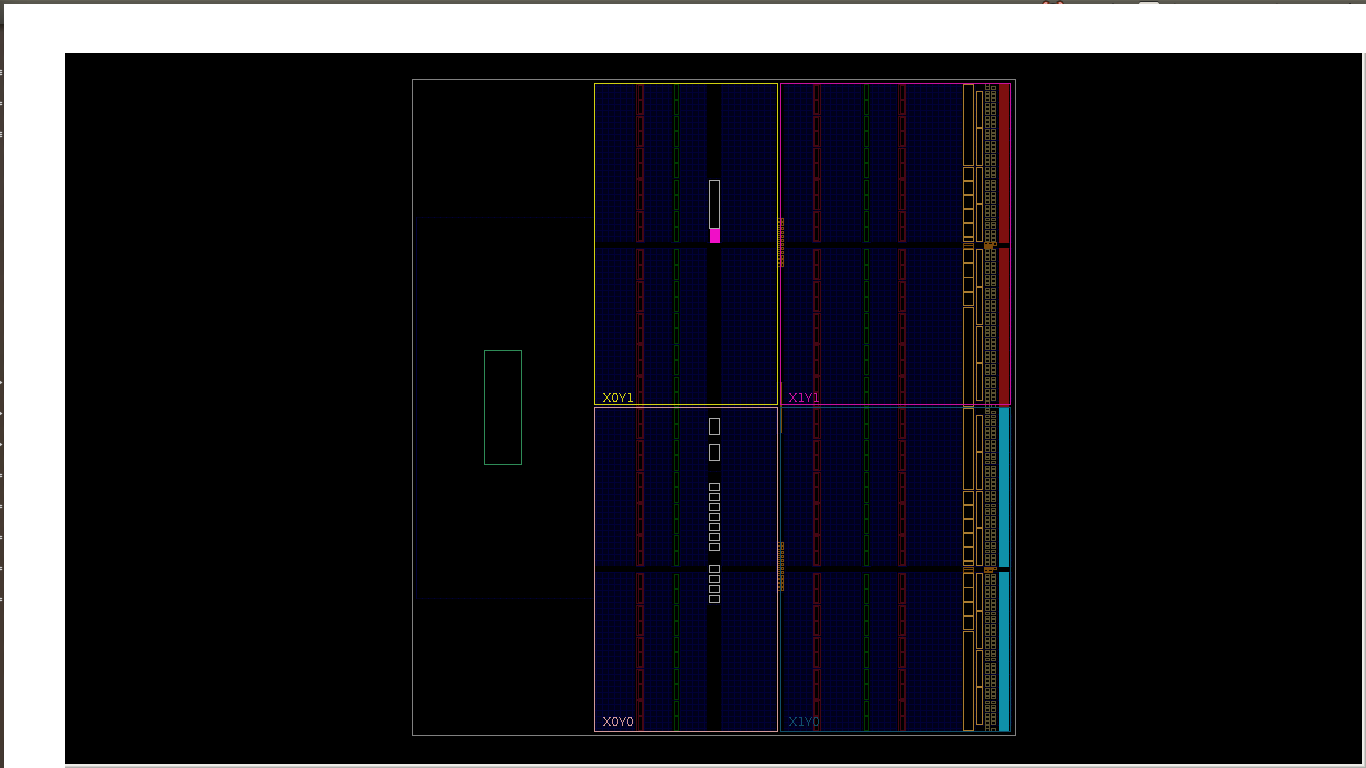
\includegraphics[width=\textwidth, height=8cm]{graphics/fpga_1.png} \\ \\

The number of BRAMs on the x axis of the FPGA fabric is expressed as 

\begin{equation}
A(x) = \begin{cases}
0, & \textbf{0$\leq$x$<$4}, \\
1, & \textbf{4$\leq$x$<$18}, \\
2, & \textbf{18$\leq$x$<$25}, \\
3, & \textbf{25$\leq$x$<$W},
\end{cases}
\end{equation}

meanwhile the number of BRAMs on the y axis equals 
\begin{equation}
B(y) = \begin{cases} 
y\%5, & \textbf{0$\leq$y$<$H},
\end{cases}
\end{equation}

The total number of BRAMs inside a slot S$_i$ equals to \\
\begin{equation}
BRAM(x_i,y_i,w_i,h_i) =  (A(x_i+w_i) - A(x_i)) \cdot (B(y_i+h_i) - B(y_i))
\end{equation}

The number of DSPs on the x axis of the FPGA fabric is expressed as 
\begin{equation}
C(x) = \begin{cases}
0, & \textbf{0$\leq$x$<$7}, \\
1, & \textbf{7$\leq$x$<$22}, \\
2, & \textbf{22$\leq$x$<$W},
\end{cases}
\end{equation}

meanwhile the number of DSPs on the y axis equals 
\begin{equation}
D(y) = \begin{cases} 
y\%5, & \textbf{0$\leq$y$<$H},
\end{cases}
\end{equation}

The total number of DSPs inside a slot S$_i$ equals to \\
\begin{equation}
DSP(x_i,y_i,w_i,h_i) =  (C(x_i+w_i) - C(x_i)) \cdot (D(y_i+h_i) - D(y_i))
\end{equation}					  


The number of CLB on the x axis is expressed 					  
\begin{equation}
F(x) = \begin{cases}
x, & \textbf{ 0$\leq$x$<$4}, \\
(x-1), & \textbf{4$\leq$x$<$7}, \\
(x-2), & \textbf{7$\leq$x$<$10}, \\
(x-3), & \textbf{10$\leq$x$<$15}, \\
(x-4), & \textbf{15$\leq$x$<$18}, \\
(x-5), & \textbf{18$\leq$x$<$22}, \\
(x-6), & \textbf{22$\leq$x$<$25}, \\
(x-7), & \textbf{25$\leq$x$<$W},
\end{cases}
\end{equation}

The number of CLB on the y axis is expressed as 
\begin{equation}
G(y) =  \begin{cases}
y, & \textbf{0$\leq$y$<$H}
\end{cases}
\end{equation}

The total number of CLBs inside a slot S$_i$ equals to \\
\begin{equation}
CLB(x_i,y_i,w_i,h_i) =  (F(x_i+w_i) - F(x_i)) \cdot (G(y_i+h_i) - G(y_i))
\end{equation}					  
			  
					  
\hspace{15mm} where \[y_i\in \{0, H-1 \}  \quad and \quad x_i\in \{0, W-1 \} \] \\

\section{Design}
\subsection{optimization variables}
To encode the ILP/MILP formulation the following binary and real variables are defined. \\
For each slot S$_i$
\begin{itemize}
\item x$_i$, y$_i$ w$_i$, h$_i$ represent the bottom left coordinates, the width and the height of the rectangle respectively
\end{itemize}

For two slots S$_i$ and S$_k$ 
\begin{itemize}
\item $\gamma_{ik}$ $\in$ [0,1] is a binary variable used to identify whether S$_i$ is found on the left or the right of S$_k$\\
$\gamma_{ik}$ = 1 if x$_i$ $\leq$ x$_k$ [i.e. S$_i$ is on the left of S$_k$]
\item $\theta_{ik}$ $\in$ [0,1] is a binary variable used to identify whether S$_i$ is found on the top or bottom of of S$_k$\\
$\theta_{ik}$ = 1 if y$_i$ $\leq$ y$_k$ [i.e. S$_i$ is found below S$_k$]
\item $\Delta_{ik}$ $\in$ [0,1] is a binary variable which indicates interfernce between slots S$_i$ and S$_k$.\\
$\Delta_{ik}$ = 0 if there is no interference between the slots [i.e. not a single tile is shared between slots]
\item D$_{w}$, B$_w$ and C$_w$ represent wasted DSPs, BRAMs and CLBs in S$_i$ respectively
\item $\alpha_i$ is a real variable that is used to express the bound on the amount of wasted resources in a slot S$_i$
\item $\rho$ and $\nu$ are vectors which contain the x and y coordinates of all the forbidden columns and rows on the FPGA fabric respectively 
\item $\eta_{ik}$ is a real variable that expresses the bound on the wirelength between S$_i$ and S$_k$
\end{itemize}


Slots for partial reconfiguration should fulfill the following constraints
\begin{itemize}
\item there must be enough resources within the slots
\item A frame can not be shared between two reconfigurable partitions (no interference)
\item static resources on the FPGA must not be included in the slots 
\item Left and right edges of slots must be placed in proper positions
\item the amount of wasted resources should be minimized (Wasting DSPs is more expensive than BRAMs which in turn is more expensive than CLBs)
\item Other optimizations such as lower wire length between slots or lower length to I/O etc... can be added as constraints
\end{itemize}

\textbf{constraint 1}: Each slot must incorporate enough resources. \\
For slot S$_i$
\begin{equation}
\begin{split}
CLB(x_{i}, y_{i}, w_{i}, h_{i}) \geq  C_{i}\\
DSP(x_{i}, y_{i}, w_{i}, h_{i}) \geq  D_{i} \\	
BRAM(x_{i}, y_{i}, w_{i}, h_{i}) \geq  B_{i}
\end{split}
\end{equation}

\textbf{Constraint 2}: A frame (tile) is the smallest reconfigurable physical region and it spans one clock region high and one resource type wide. A Reconfigurable Frame can not contain logic from more than one Reconfigurable Partition. Two slots S$_1$ \{x$_1$, y$_1$, w$_1$, h$_1$\} and S$_2$\{ x$_2$, y$_2$, w$_2$, h$_2$ \} do not interfere i.e. do not have at least one common tile between them, under the following conditions \\

\begin{algorithmic}
\IF{x$_1$ $\leq$ x$_2$ and y$_1$ $\leq$ y$_2$}
	\STATE x$_1$ + w$_1$ $<$ x$_2$ or y$_1$ + h$_1$ $<$ y$_2$
\ELSIF {x$_1$ $\geq$ x$_2$ and y$_1$ $\geq$ y$_2$}
	\STATE x$_2$ + w$_2$ $<$ x$_1$ or y$_2$ + h$_2$ $<$ y$_1$
\ELSIF {x$_1$ $<$ x$_2$ and y$_1$ $>$ y$_2$}
	\STATE x$_1$ + w$_1$ $<$ x$_2$ or y$_2$ + h$_2$ $<$ y$_1$
\ELSE
	\STATE x$_2$ + w$_2$ $<$ x$_2$ or y$_1$ + h$_1$ $<$ y$_2$
\ENDIF
\end{algorithmic}

Hence using the conditions above $\Delta_{ik}$ which is used to test interference between slots S$_i$ and S$_k$ is expressed as
\begin{equation}
\begin{split}
\Delta_{ik} = \gamma_{ik}(1-(x_k-x_i-w_i)) \cdot \theta(1-(y_k-y_i-h_i))  \quad + \\
			   	(1-\gamma_{ik})(1-(x_i-x_k-w_k)) \cdot (1-\theta_{ik})(1-(y_i-y_k-h_k))\quad  + \\
			   \gamma_{ik}(1-(x_k-x	_i-w_i)) \cdot (1-\theta_{ik})(1-(y_i-y_k-h_k))\quad + \\
			   (1-\gamma_{ik})(1-(x_i-x_k-h_k)) \cdot \theta(1-(y_k-y_i-h_i)) 
\end{split}
\end{equation}

Therefore for N slots on an FPGA it can be said that slot S$_i$ faces no interferance from the N-1 slots if
\begin{equation}
\sum_{k=1}^{N-1} \Delta_{ik} = 0
\end{equation}  
 
\textbf{constraint 3}: Global resources, clock resources (central clock column, BUFG, BUFR, MMCM etc...), static components (BSCAN, ICAP, XADC etc...) must not be included in the rectangles. The $\rho$ and $\nu$ vectors contain the x and y coordinates of these resources on the FPGA fabric. These resources are not included in a slot S$_i$ if 
\begin{equation}
\begin{split}
(x_i, x_i+w_i) \notin \rho \\
(y_i, y_i+h_i) \notin \nu
\end{split}
\end{equation}

\textbf{constraint 4}: The left and right edges of the rectangles must be placed between CLB-CLB, CLB-BRAM or CLB-DSP and not between two interconnect columns (INT-INT).

\textbf{constraint 5}: The number of wasted resources in a slot S$_i$ must be bounded. Resources are considered wasted if they are included in a slot while not being used.  The wasted resources D$_{w}$, B$_w$ and C$_w$ in slot S$_i$ can be calculated as
\begin{equation}
\begin{split}
D_w = D_i - DSP(x_i, y_i, w_i, h_i) \\
B_w = B_i - BRAM(x_i, y_i, w_i, h_i) \\
C_w = C_i - CLB(x_i, y_i, w_i, h_i) \\ 
\end{split}
\end{equation}

Hence the constraint on wasted resources in S$_i$ can be expressed as 
\begin{equation}
\alpha_i \leq (\phi_d \cdot D_w) + (\phi_b \cdot B_w) + (\phi_c \cdot C_w)
\end{equation}
where $\phi_d$, $\phi_b$ and $\phi_c$ are the weights which signify the importance of resources. All FPGA resources are not equally valuable hence wasting DSPs is worse than BRAMs which in turn is worse than CLBs. Accordingly 
\begin{equation}
\phi_d > \phi_b > \phi_c
\end{equation}

\textbf{constraint 6}: Other constraints such as minimal wire length between slots (to reduce routing delay and power consumption) can be used as constraints to choose the optimal slots \\

\end{document}